\documentclass[../PianoDiProgetto.tex]{subfiles}
\begin{document}

\section{Preventivo}
	\subsection{Stima}
		\subsubsection{Fase 1}
			\paragraph{Suddivisione del lavoro}
			Ogni componente del gruppo \kpanic\ rivestirà i seguenti ruoli:
			\begin{table}[h]
				%\centering
				\begin{tabularx}{\textwidth}{l * {6}{C} c}
				\toprule
				\textbf{Nominativo} & \textbf{Rp} & \textbf{Am} & \textbf{Pt} & \textbf{An} & \textbf{Pm} & \textbf{Ve} & \textbf{Ore totali} \\
				\midrule
				Berto Filippo &	0 & 13 & 0 & 12 & 0 & 5 & 30 \\
				%\midrule
				Fasolato Francesco & 9 & 9 & 0 & 0 & 0 & 12 & 30 \\
				%\midrule
				Favaro Daniele & 12 & 0 & 0 & 12 & 0 & 6 & 30 \\
				%\midrule
				Franceschini Marco & 0 & 9 & 0 & 12 & 0 & 9 & 30 \\
				%\midrule
				Macrì Antonino & 11 & 8 & 0 & 7 & 0 & 4 & 30 \\
				%\midrule
				Zanon Edoardo &	0 & 14 & 0 & 11 & 0 & 5 & 30 \\
				%\midrule
				Zecchin Giacomo & 0 & 11 & 0 & 14 & 0 & 5 & 30 \\
				\midrule			
				\textbf{Ore Totali Ruolo} & 32 & 64 & 0 & 68 & 0 & 46 & 210 \\
				\bottomrule
				\end{tabularx}
				\caption{Fase 1 - Suddivisione delle ore di lavoro}		
			\end{table}

			Riassumendo la precedente tabella con un bar chart:	
			\begin{figure}[!h]
				\centering
				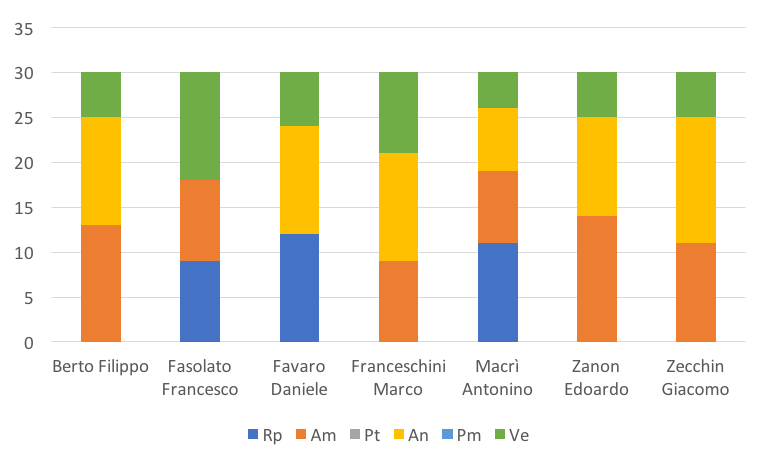
\includegraphics[width=\textwidth]{Preventivo/Immagini/fase1_oreRuoloPersona.png}
				\caption{Fase 1 - Riassunto ore di lavoro per persona}
			\end{figure}	
			
			\newpage
			\paragraph{Prospetto economico}
			Il costo di ogni ruolo è indicato di seguito:
			\begin{table}[h]
				\centering
				\begin{tabular}{l * {2}{c}}
				\toprule
				\textbf{Ruolo} & \textbf{Ore} & \textbf{Costo (\euro{})} \\
				\midrule
				Responsabile & 32 & 960,00 \\
				%\midrule
				Amministratore & 64 & 1.280,00 \\
				%\midrule
				Progettista & 0 & 0,00 \\
				%\midrule
				Analista & 68 & 1.700,00 \\		
				%\midrule
				Programmatore & 0 & 0,00 \\		
				%\midrule
				Verificatore & 46 & 690,00 \\				
				\midrule		
				\textbf{Totale} & 210 & 4.630,00 \\
				\bottomrule	
				\end{tabular}
				\caption{Fase 1 - Prospetto economico}		
			\end{table}
			
			Riassumendo la precedente tabella con due pie chart:	
			\begin{figure}[!h]
				\centering
				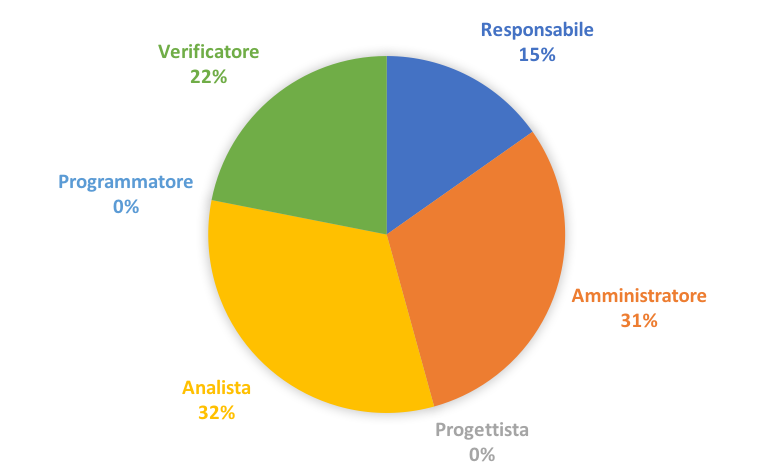
\includegraphics[width=\textwidth]{Preventivo/Immagini/fase1_oreRuolo.png}
				\caption{Fase 1 - Riassunto ore di lavoro per ruolo}
			\end{figure}	
			\newpage
			\begin{figure}[!h]
				\centering
				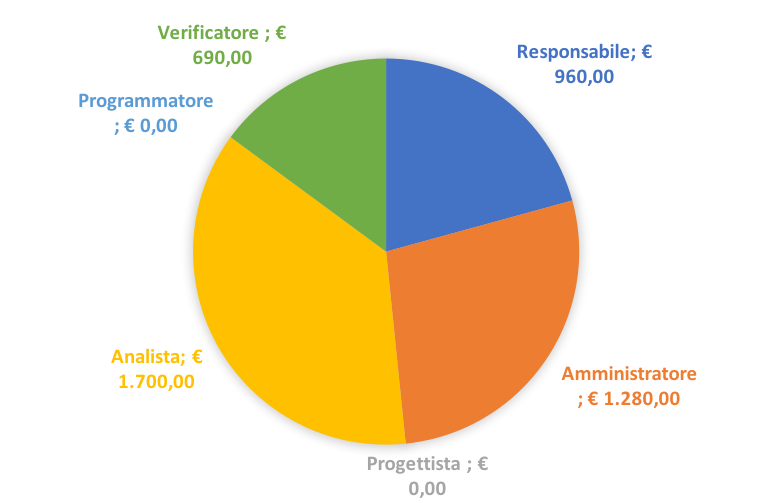
\includegraphics[width=\textwidth]{Preventivo/Immagini/fase1_costoRuolo.png}
				\caption{Fase 1 - Riassunto costo per ruolo}
			\end{figure}	
			
		\newpage			
		\subsubsection{Fase 2}
			\paragraph{Suddivisione del lavoro}
			Ogni componente del gruppo \kpanic\ rivestirà i seguenti ruoli:
			\begin{table}[h]
				%\centering
				\begin{tabularx}{\textwidth}{l * {6}{C} c}
				\toprule
				\textbf{Nominativo} & \textbf{Rp} & \textbf{Am} & \textbf{Pt} & \textbf{An} & \textbf{Pm} & \textbf{Ve} & \textbf{Ore totali} \\
				\midrule
				Berto Filippo &	0 & 0 & 0 & 4 & 0 & 5 & 9 \\
				%\midrule
				Fasolato Francesco & 0 & 5 & 0 & 4 & 0 & 0 & 9 \\
				%\midrule
				Favaro Daniele & 0 & 4 & 0 & 0 & 0 & 6 & 10 \\
				%\midrule
				Franceschini Marco & 0 & 0 & 0 & 3 & 0 & 6 & 9 \\
				%\midrule
				Macrì Antonino & 0 & 0 & 0 & 4 & 0 & 5 & 9 \\
				%\midrule
				Zanon Edoardo &	5 & 0 & 0 & 3 & 0 & 2 & 10 \\
				%\midrule
				Zecchin Giacomo & 4 & 0 & 0 & 0 & 0 & 6 & 10 \\
				\midrule			
				\textbf{Ore Totali Ruolo} & 9 & 9 & 0 & 18 & 0 & 30 & 66 \\
				\bottomrule
				\end{tabularx}
				\caption{Fase 2 - Suddivisione delle ore di lavoro}		
			\end{table}
			
			Riassumendo la precedente tabella con un bar chart:	
			\begin{figure}[!h]
				\centering
				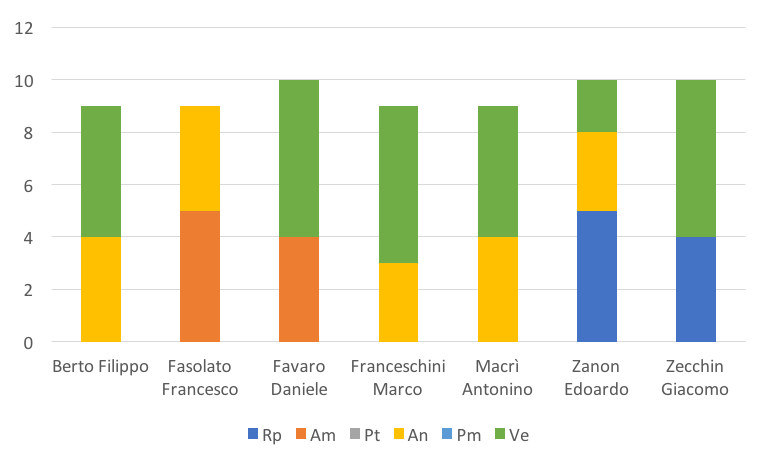
\includegraphics[width=\textwidth]{Preventivo/Immagini/fase2_oreRuoloPersona.png}
				\caption{Fase 2 - Riassunto ore di lavoro per persona}
			\end{figure}	
			
			\newpage
			\paragraph{Prospetto economico}
			Il costo di ogni ruolo è indicato di seguito:
			\begin{table}[h]
				\centering
				\begin{tabular}{l * {2}{c}}
				\toprule
				\textbf{Ruolo} & \textbf{Ore} & \textbf{Costo (\euro{})} \\
				\midrule
				Responsabile & 9 & 270,00 \\
				%\midrule
				Amministratore & 9 & 180,00 \\
				%\midrule
				Progettista & 0 & 0,00 \\
				%\midrule
				Analista & 18 & 450,00 \\		
				%\midrule
				Programmatore & 0 & 0,00 \\		
				%\midrule
				Verificatore & 30 & 450,00 \\				
				\midrule		
				\textbf{Totale} & 66 & 1.350,00 \\
				\bottomrule	
				\end{tabular}
				\caption{Fase 2 - Prospetto economico}		
			\end{table}
			
			Riassumendo la precedente tabella con due pie chart:	
			\begin{figure}[!h]
				\centering
				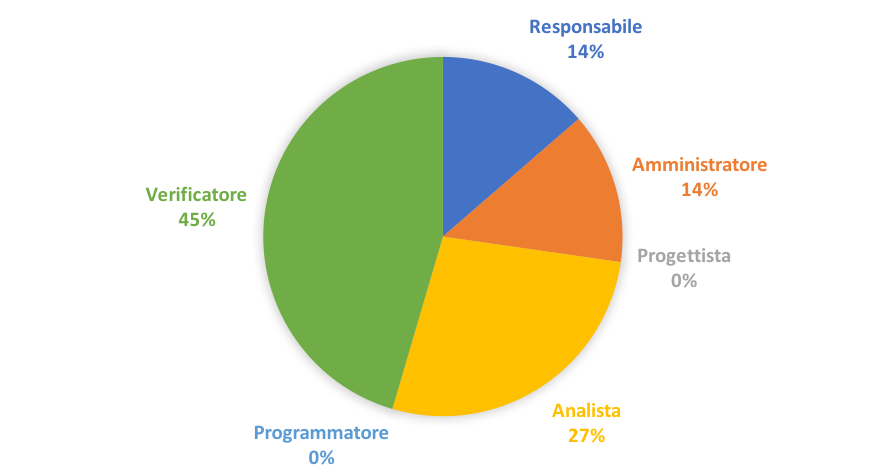
\includegraphics[width=\textwidth]{Preventivo/Immagini/fase2_oreRuolo.png}
				\caption{Fase 2 - Riassunto ore di lavoro per ruolo}
			\end{figure}	
			\newpage
			\begin{figure}[!h]
				\centering
				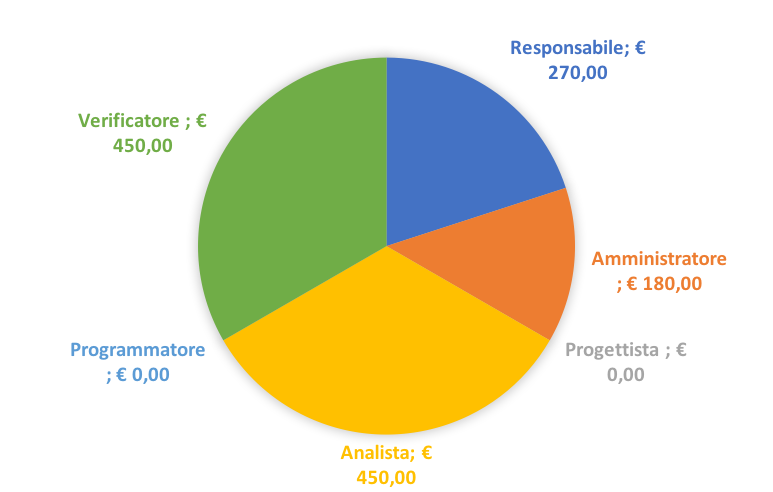
\includegraphics[width=\textwidth]{Preventivo/Immagini/fase2_costoRuolo.png}
				\caption{Fase 2 - Riassunto costo per ruolo}
			\end{figure}	
			
		\newpage
		\subsubsection{Fase 3}
			\paragraph{Suddivisione del lavoro}
			Ogni componente del gruppo \kpanic\ rivestirà i seguenti ruoli:
			\begin{table}[h]
				%\centering
				\begin{tabularx}{\textwidth}{l * {6}{C} c}
				\toprule
				\textbf{Nominativo} & \textbf{Rp} & \textbf{Am} & \textbf{Pt} & \textbf{An} & \textbf{Pm} & \textbf{Ve} & \textbf{Ore totali} \\
				\midrule
				Berto Filippo &	0 & 0 & 18 & 7 & 0 & 0 & 25 \\
				%\midrule
				Fasolato Francesco & 0 & 0 & 17 & 0 & 0 & 7 & 24 \\
				%\midrule
				Favaro Daniele & 0 & 0 & 17 & 0 & 0 & 7 & 24 \\
				%\midrule
				Franceschini Marco & 18	& 0 & 0 & 0 & 0 & 7 & 25 \\
				%\midrule
				Macrì Antonino & 0 & 8 & 0 & 11 & 0 & 5 & 24 \\
				%\midrule
				Zanon Edoardo &	0	& 0 & 18 & 7 & 0	 & 0 & 25 \\
				%\midrule
				Zecchin Giacomo & 0 & 8 & 0 & 11 & 0 & 5 & 24 \\
				\midrule			
				\textbf{Ore Totali Ruolo} & 18 & 16 & 70 & 36 & 0 & 31 & 171 \\
				\bottomrule
				\end{tabularx}
				\caption{Fase 3 - Suddivisione delle ore di lavoro}		
			\end{table}
			
			Riassumendo la precedente tabella con un bar chart:	
			\begin{figure}[!h]
				\centering
				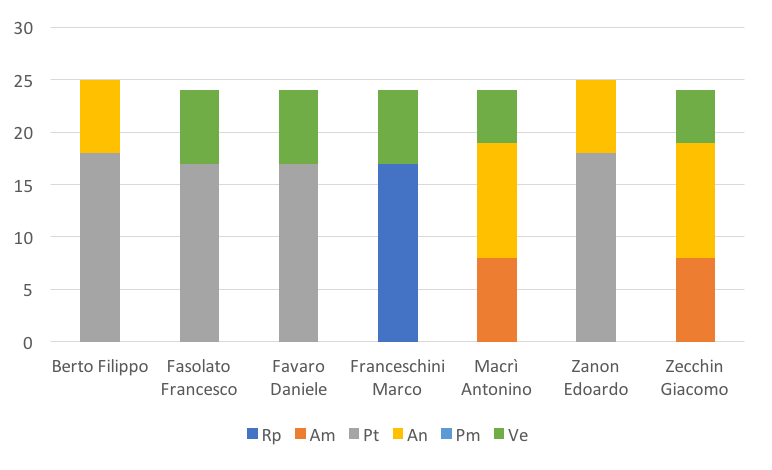
\includegraphics[width=\textwidth]{Preventivo/Immagini/fase3_oreRuoloPersona.png}
				\caption{Fase 3 - Riassunto ore di lavoro per persona}
			\end{figure}	
			
			\newpage
			\paragraph{Prospetto economico}
			Il costo di ogni ruolo è indicato di seguito:
			\begin{table}[h]
				\centering
				\begin{tabular}{l * {2}{c}}
				\toprule
				\textbf{Ruolo} & \textbf{Ore} & \textbf{Costo (\euro{})} \\
				\midrule
				Responsabile & 18 & 540,00 \\
				%\midrule
				Amministratore & 16 & 320,00 \\
				%\midrule
				Progettista & 70 & 1.540,00 \\
				%\midrule
				Analista & 36 & 900,00 \\		
				%\midrule
				Programmatore & 0 & 0,00 \\		
				%\midrule
				Verificatore & 31 & 465,00 \\				
				\midrule		
				\textbf{Totale} & 171 & 3.765,00 \\
				\bottomrule	
				\end{tabular}
				\caption{Fase 3 - Prospetto economico}		
			\end{table}
			
			Riassumendo la precedente tabella con due pie chart:	
			\begin{figure}[!h]
				\centering
				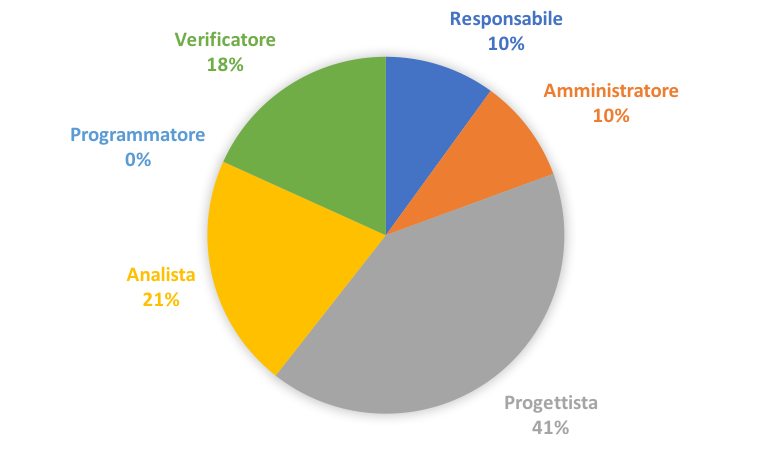
\includegraphics[width=\textwidth]{Preventivo/Immagini/fase3_oreRuolo.png}
				\caption{Fase 3 - Riassunto ore di lavoro per ruolo}
			\end{figure}
			\newpage
			\begin{figure}[!h]
				\centering
				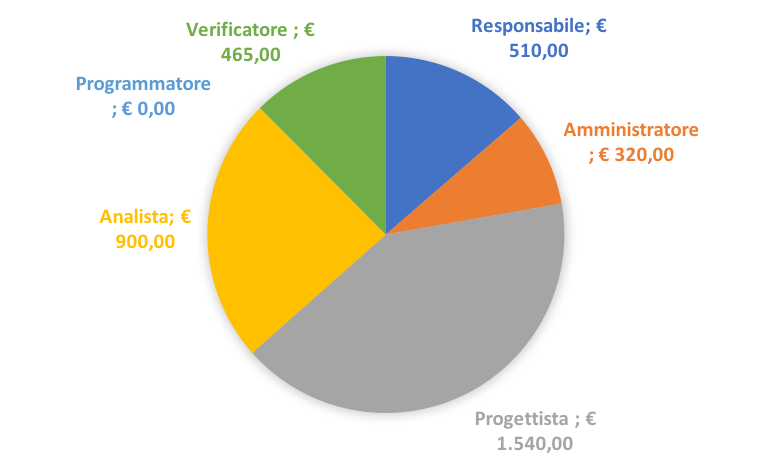
\includegraphics[width=\textwidth]{Preventivo/Immagini/fase3_costoRuolo.png}
				\caption{Fase 3 - Riassunto costo per ruolo}
			\end{figure}		

		\newpage
		\subsubsection{Fase 4}
			\paragraph{Suddivisione del lavoro}
			Ogni componente del gruppo \kpanic\ rivestirà i seguenti ruoli:
			\begin{table}[h]
				%\centering
				\begin{tabularx}{\textwidth}{l * {6}{C} c}
				\toprule
				\textbf{Nominativo} & \textbf{Rp} & \textbf{Am} & \textbf{Pt} & \textbf{An} & \textbf{Pm} & \textbf{Ve} & \textbf{Ore totali} \\
				\midrule
				Berto Filippo &	16 & 0 & 0 & 0 & 12 & 0 & 28 \\
				%\midrule
				Fasolato Francesco & 0 & 7 & 0 & 8 & 0 & 13 & 28 \\
				%\midrule
				Favaro Daniele & 0 & 0 & 0 & 0 & 13 & 16 & 29 \\
				%\midrule
				Franceschini Marco & 0 & 0 & 11 &	0 & 18 & 0 & 29 \\
				%\midrule
				Macrì Antonino & 0 & 7 & 16 & 0 & 0 & 5 & 28 \\
				%\midrule
				Zanon Edoardo &	0 & 0 & 11 & 0 & 16 & 0	 & 27 \\
				%\midrule
				Zecchin Giacomo & 0 & 0 & 11 & 0 & 18 & 0 & 29 \\
				\midrule			
				\textbf{Ore Totali Ruolo} & 16 & 14 & 49 & 8 & 77 & 34 & 198 \\
				\bottomrule
				\end{tabularx}
				\caption{Fase 4 - Suddivisione delle ore di lavoro}		
			\end{table}
			
			Riassumendo la precedente tabella con un bar chart:	
			\begin{figure}[!h]
				\centering
				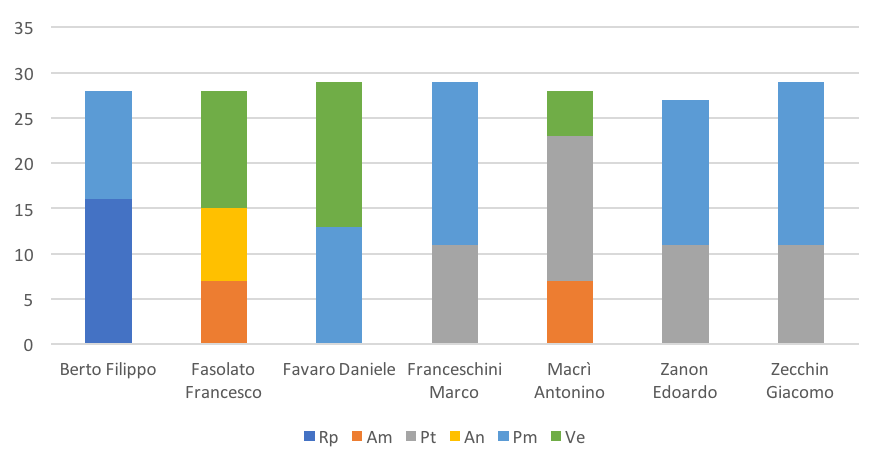
\includegraphics[width=\textwidth]{Preventivo/Immagini/fase4_oreRuoloPersona.png}
				\caption{Fase 4 - Riassunto ore di lavoro per persona}
			\end{figure}	
			
			\newpage
			\paragraph{Prospetto economico}
			Il costo di ogni ruolo è indicato di seguito:
			\begin{table}[h]
				\centering
				\begin{tabular}{l * {2}{c}}
				\toprule
				\textbf{Ruolo} & \textbf{Ore} & \textbf{Costo (\euro{})} \\
				\midrule
				Responsabile & 16 & 480,00 \\
				%\midrule
				Amministratore & 14 & 280,00 \\
				%\midrule
				Progettista & 49 & 1.078,00 \\
				%\midrule
				Analista & 8 & 200,00 \\		
				%\midrule
				Programmatore & 77 & 1.155,00 \\		
				%\midrule
				Verificatore & 34 & 510,00 \\				
				\midrule		
				\textbf{Totale} & 198 & 3.703,00 \\
				\bottomrule	
				\end{tabular}
				\caption{Fase 4 - Prospetto economico}		
			\end{table}
			
			Riassumendo la precedente tabella con due pie chart:	
			\begin{figure}[!h]
				\centering
				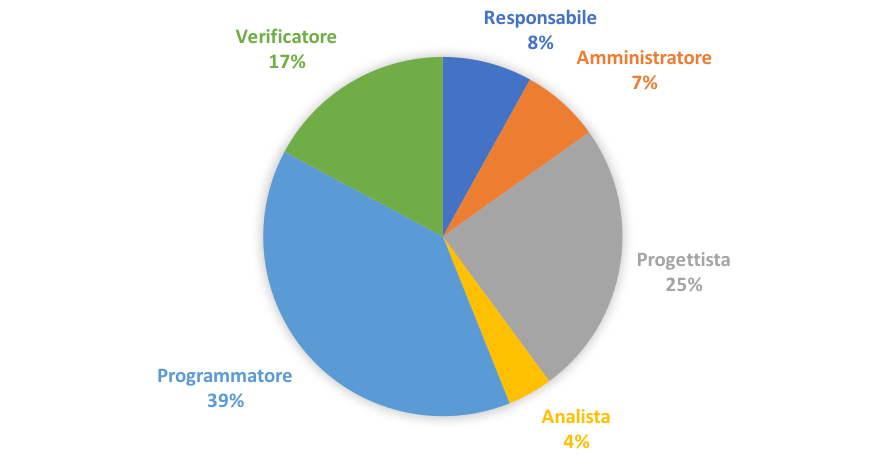
\includegraphics[width=\textwidth]{Preventivo/Immagini/fase4_oreRuolo.png}
				\caption{Fase 4 - Riassunto ore di lavoro per ruolo}
			\end{figure}	
			\newpage
			\begin{figure}[!h]
				\centering
				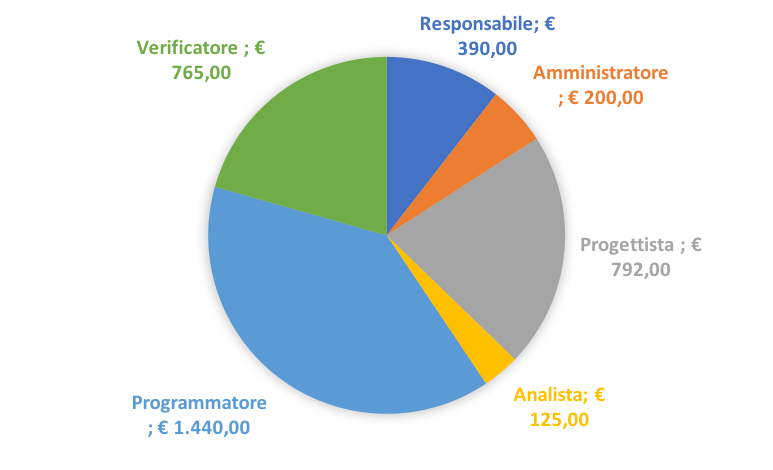
\includegraphics[width=\textwidth]{Preventivo/Immagini/fase4_costoRuolo.png}
				\caption{Fase 4 - Riassunto costo per ruolo}
			\end{figure}	
		
		\newpage
		\subsubsection{Fase 5}
			\paragraph{Suddivisione del lavoro}
			Ogni componente del gruppo \kpanic\ rivestirà i seguenti ruoli:
			\begin{table}[h]
				%\centering
				\begin{tabularx}{\textwidth}{l * {6}{C} c}
				\toprule
				\textbf{Nominativo} & \textbf{Rp} & \textbf{Am} & \textbf{Pt} & \textbf{An} & \textbf{Pm} & \textbf{Ve} & \textbf{Ore totali} \\
				\midrule
				Berto Filippo &	0 & 0 & 0 & 5 & 0 & 9 & 14 \\
				%\midrule
				Fasolato Francesco & 0 & 0 & 6 & 3 & 0 & 7 & 16 \\
				%\midrule
				Favaro Daniele & 0 & 6 & 0 & 5 & 0 & 5 & 16 \\
				%\midrule
				Franceschini Marco & 0 & 0 & 0 & 0 & 10 & 5 & 15 \\
				%\midrule
				Macrì Antonino & 0 & 0 & 0 & 0 & 10 & 4 & 14 \\
				%\midrule
				Zanon Edoardo &	10 & 0 & 0 & 0 & 0 & 6 & 16 \\
				%\midrule
				Zecchin Giacomo & 0 & 0 & 6 & 0 & 0 & 8 & 14 \\
				\midrule			
				\textbf{Ore Totali Ruolo} & 10 & 6 & 12 & 13 & 20 & 44 & 105 \\
				\bottomrule
				\end{tabularx}
				\caption{Fase 5 - Suddivisione delle ore di lavoro}		
			\end{table}

			Riassumendo la precedente tabella con un bar chart:	
			\begin{figure}[!h]
				\centering
				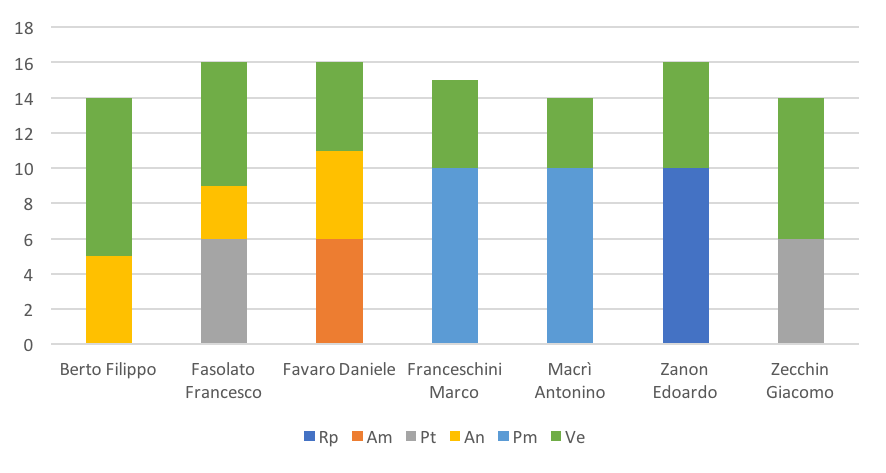
\includegraphics[width=\textwidth]{Preventivo/Immagini/fase5_oreRuoloPersona.png}
				\caption{Fase 5 - Riassunto ore di lavoro per persona}
			\end{figure}	
			
			\newpage
			\paragraph{Prospetto economico}
			Il costo di ogni ruolo è indicato di seguito:
			\begin{table}[h]
				\centering
				\begin{tabular}{l * {2}{c}}
				\toprule
				\textbf{Ruolo} & \textbf{Ore} & \textbf{Costo (\euro{})} \\
				\midrule
				Responsabile & 10 & 300,00 \\
				%\midrule
				Amministratore & 6 & 120,00 \\
				%\midrule
				Progettista & 12 & 264,00 \\
				%\midrule
				Analista & 13 & 325,00 \\		
				%\midrule
				Programmatore & 20 & 300,00 \\		
				%\midrule
				Verificatore & 44 & 660,00 \\				
				\midrule		
				\textbf{Totale} & 105 & 1.969,00 \\
				\bottomrule	
				\end{tabular}
				\caption{Fase 5 - Prospetto economico}		
			\end{table}
			
			Riassumendo la precedente tabella con due pie chart:	
			\begin{figure}[!h]
				\centering
				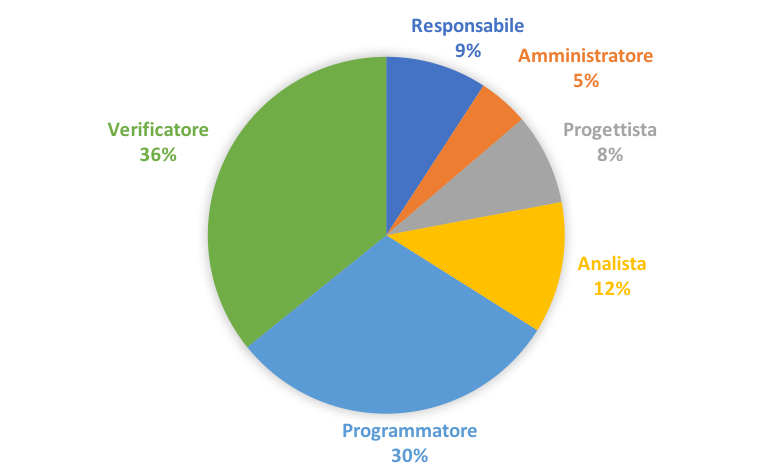
\includegraphics[width=\textwidth]{Preventivo/Immagini/fase5_oreRuolo.png}
				\caption{Fase 5 - Riassunto ore di lavoro per ruolo}
			\end{figure}
			\newpage	
			\begin{figure}[!h]
				\centering
				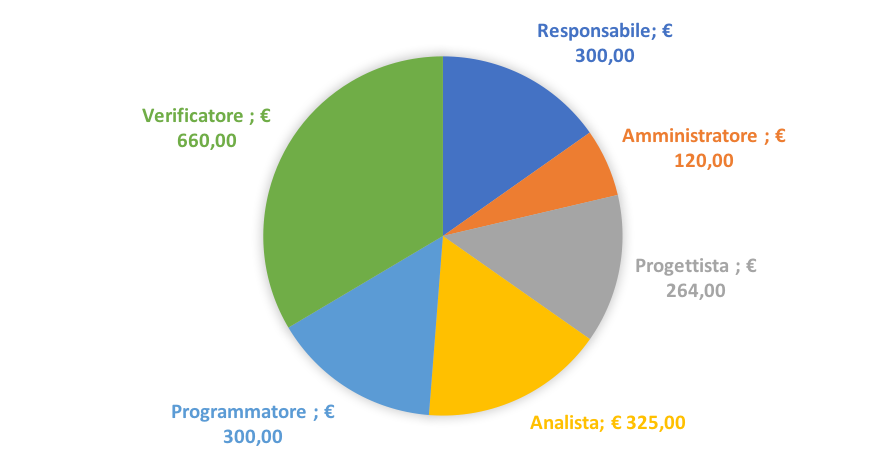
\includegraphics[width=\textwidth]{Preventivo/Immagini/fase5_costoRuolo.png}
				\caption{Fase 5 - Riassunto costo per ruolo}
			\end{figure}	
			
		\newpage
		\subsubsection{Fase 6}
			\paragraph{Suddivisione del lavoro}
			Ogni componente del gruppo \kpanic\ rivestirà i seguenti ruoli:
			\begin{table}[h]
				%\centering
				\begin{tabularx}{\textwidth}{l * {6}{C} c}
				\toprule
				\textbf{Nominativo} & \textbf{Rp} & \textbf{Am} & \textbf{Pt} & \textbf{An} & \textbf{Pm} & \textbf{Ve} & \textbf{Ore totali} \\
				\midrule
				Berto Filippo &	0 & 0 & 4 & 0 & 7 & 0 & 11 \\
				%\midrule
				Fasolato Francesco & 0 & 4 & 4 & 0 & 0 & 4 & 12 \\
				%\midrule
				Favaro Daniele & 0 & 0 & 5 & 0 & 0 & 6 & 11 \\
				%\midrule
				Franceschini Marco & 0& 0 & 4 & 0 & 0 & 5 & 9 \\
				%\midrule
				Macrì Antonino & 0 & 0 & 0 & 0 & 10 & 4 & 14 \\
				%\midrule
				Zanon Edoardo &	0 &0 & 0 & 0 & 6 & 5 & 11 \\
				%\midrule
				Zecchin Giacomo & 5 & 0 & 5 & 0 & 0 & 0 & 10 \\
				\midrule			
				\textbf{Ore Totali Ruolo} & 5 & 7 & 22 & 5 & 13 & 23 & 75 \\
				\bottomrule
				\end{tabularx}
				\caption{Fase 6 - Suddivisione delle ore di lavoro}		
			\end{table}
			
			Riassumendo la precedente tabella con un bar chart:	
			\begin{figure}[!h]
				\centering
				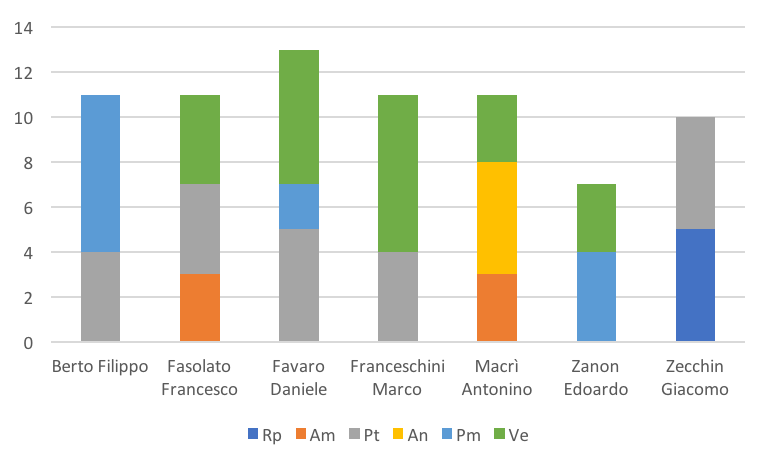
\includegraphics[width=\textwidth]{Preventivo/Immagini/fase6_oreRuoloPersona.png}
				\caption{Fase 6 - Riassunto ore di lavoro per persona}
			\end{figure}	

			\newpage
			\paragraph{Prospetto economico}
			Il costo di ogni ruolo è indicato di seguito:
			\begin{table}[h]
				\centering
				\begin{tabular}{l * {2}{c}}
				\toprule
				\textbf{Ruolo} & \textbf{Ore} & \textbf{Costo (\euro{})} \\
				\midrule
				Responsabile & 5 & 150,00 \\
				%\midrule
				Amministratore & 7 & 140,00 \\
				%\midrule
				Progettista & 22 & 484,00 \\
				%\midrule
				Analista & 5 & 125,00 \\		
				%\midrule
				Programmatore & 13 & 195,00 \\		
				%\midrule
				Verificatore & 23 & 345,00 \\				
				\midrule		
				\textbf{Totale} & 75 & 1.439,00 \\
				\bottomrule	
				\end{tabular}
				\caption{Fase 6 - Prospetto economico}		
			\end{table}
			
			Riassumendo la precedente tabella con due pie chart:	
			\begin{figure}[!h]
				\centering
				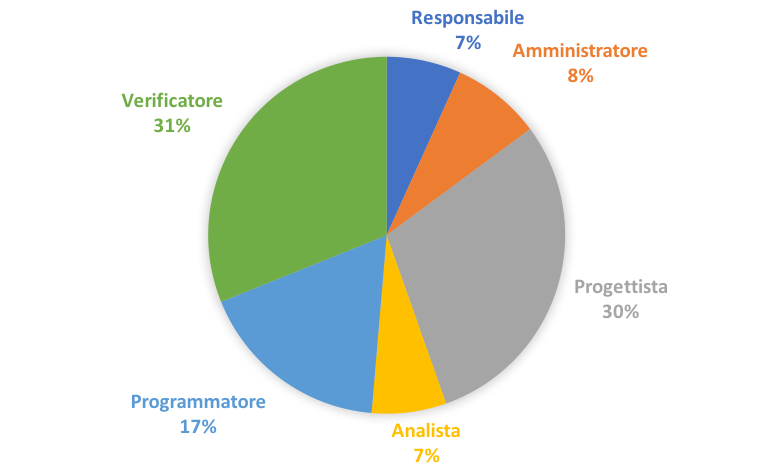
\includegraphics[width=\textwidth]{Preventivo/Immagini/fase6_oreRuolo.png}
				\caption{Fase 6 - Riassunto ore di lavoro per ruolo}
			\end{figure}	
			\newpage
			\begin{figure}[!h]
				\centering
				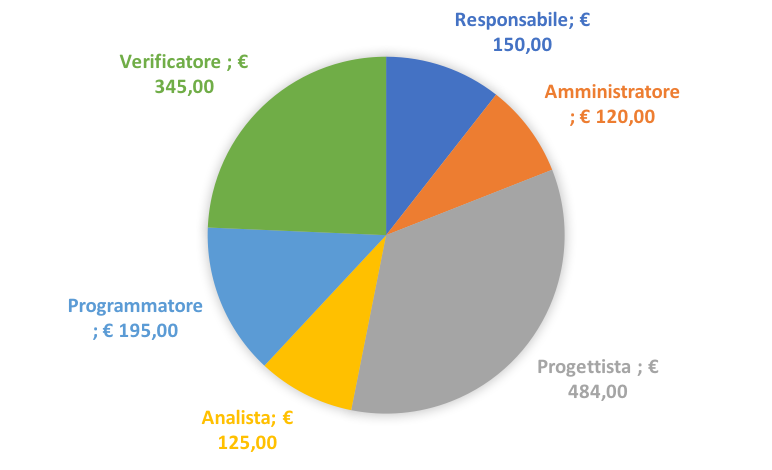
\includegraphics[width=\textwidth]{Preventivo/Immagini/fase6_costoRuolo.png}
				\caption{Fase 6 - Riassunto costo per ruolo}
			\end{figure}	

		\newpage
		\subsubsection{Fase 7}
			\paragraph{Suddivisione del lavoro}
			Ogni componente del gruppo \kpanic\ rivestirà i seguenti ruoli:
			\begin{table}[h]
				%\centering
				\begin{tabularx}{\textwidth}{l * {6}{C} c}
				\toprule
				\textbf{Nominativo} & \textbf{Rp} & \textbf{Am} & \textbf{Pt} & \textbf{An} & \textbf{Pm} & \textbf{Ve} & \textbf{Ore totali} \\
				\midrule
				Berto Filippo &	0 & 4 & 0 & 0 & 10 & 0 & 14 \\
				%\midrule
				Fasolato Francesco & 0 & 0 & 0 & 0 & 8 & 4 & 12 \\
				%\midrule
				Favaro Daniele & 0 & 0 & 0 & 0 & 0 & 11 & 11 \\
				%\midrule
				Franceschini Marco & 0 & 0 & 7 & 0 & 0 & 7 & 14 \\
				%\midrule
				Macrì Antonino & 0 & 0 & 7 & 0 & 0 & 8 & 15 \\
				%\midrule
				Zanon Edoardo &	5 & 0 & 0 & 0 & 0 & 7 & 12 \\
				%\midrule
				Zecchin Giacomo & 6 & 0 & 0 & 0 & 0 & 8 & 14 \\
				\midrule			
				\textbf{Ore Totali Ruolo} & 11 & 4 & 14 & 0 & 18 & 45 & 92 \\
				\bottomrule
				\end{tabularx}
				\caption{Fase 7 - Suddivisione delle ore di lavoro}		
			\end{table}
			
			Riassumendo la precedente tabella con un bar chart:	
			\begin{figure}[!h]
				\centering
				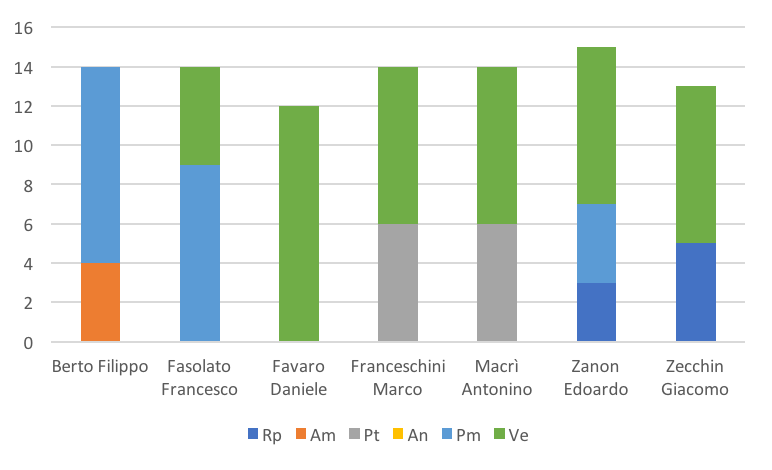
\includegraphics[width=\textwidth]{Preventivo/Immagini/fase7_oreRuoloPersona.png}
				\caption{Fase 7 - Riassunto ore di lavoro per persona}
			\end{figure}	

			\newpage
			\paragraph{Prospetto economico}
			Il costo di ogni ruolo è indicato di seguito:
			\begin{table}[h]
				\centering
				\begin{tabular}{l * {2}{c}}
				\toprule
				\textbf{Ruolo} & \textbf{Ore} & \textbf{Costo (\euro{})} \\
				\midrule
				Responsabile & 11 & 330,00 \\
				%\midrule
				Amministratore & 4 & 80,00 \\
				%\midrule
				Progettista & 14 & 308,00 \\
				%\midrule
				Analista & 0 & 0,00 \\		
				%\midrule
				Programmatore & 18 & 270,00 \\		
				%\midrule
				Verificatore & 45 & 675,00 \\				
				\midrule		
				\textbf{Totale} & 92 & 1.663,00 \\
				\bottomrule	
				\end{tabular}
				\caption{Fase 7 - Prospetto economico}		
			\end{table}
			
			Riassumendo la precedente tabella con due pie chart:	
			\begin{figure}[!h]
				\centering
				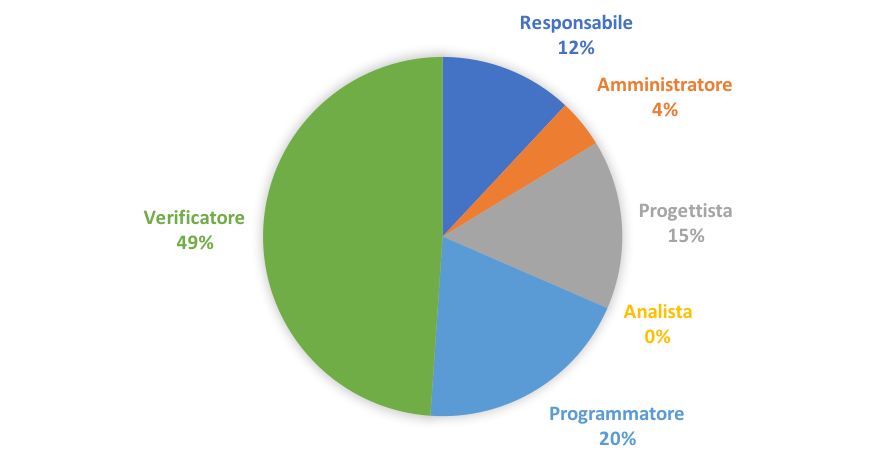
\includegraphics[width=\textwidth]{Preventivo/Immagini/fase7_oreRuolo.png}
				\caption{Fase 7 - Riassunto ore di lavoro per ruolo}
			\end{figure}	
			\newpage
			\begin{figure}[!h]
				\centering
				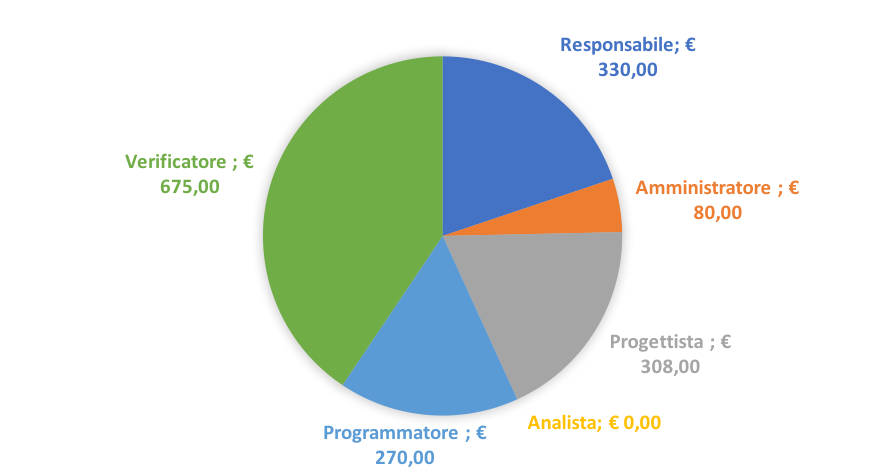
\includegraphics[width=\textwidth]{Preventivo/Immagini/fase7_costoRuolo.png}
				\caption{Fase 7 - Riassunto costo per ruolo}
			\end{figure}	

	\newpage
	\subsection{Riepilogo}
		\subsubsection{Ore totali}
			\paragraph{Suddivisione del lavoro}
			Vengono riportate le ore totali che ogni componente del gruppo \kpanic\ dedicherà per ogni ruolo a rotazione:
			\begin{table}[h]
				%\centering
				\begin{tabularx}{\textwidth}{l * {6}{C} c}
				\toprule
				\textbf{Nominativo} & \textbf{Rp} & \textbf{Am} & \textbf{Pt} & \textbf{An} & \textbf{Pm} & \textbf{Ve} & \textbf{Ore totali} \\
				\midrule
				Berto Filippo &	16 & 17 & 22 & 28 & 29 & 19 & 131 \\
				%\midrule
				Fasolato Francesco & 9 & 25 & 27 & 15 & 8 & 47 & 131 \\
				%\midrule
				Favaro Daniele & 12 & 10 & 22 & 17 & 13 & 57 & 131 \\
				%\midrule
				Franceschini Marco & 18 & 9 & 22 & 15 & 28 & 39 & 131 \\
				%\midrule
				Macrì Antonino & 11 & 26 & 23 & 27 & 10 & 34 & 131 \\
				%\midrule
				Zanon Edoardo &	20 & 14 & 29 & 21 & 22 & 25 & 131 \\
				%\midrule
				Zecchin Giacomo & 15 & 19 & 22 & 25 & 18 & 32 & 131 \\
				\midrule			
				\textbf{Ore Totali Ruolo} & 101 & 120 & 167 & 148 & 128 & 253 & 917 \\
				\bottomrule
				\end{tabularx}
				\caption{Suddivisione delle ore totali di lavoro}		
			\end{table}

			Riassumendo la precedente tabella con un bar chart:
			\begin{figure}[!h]
				\centering
				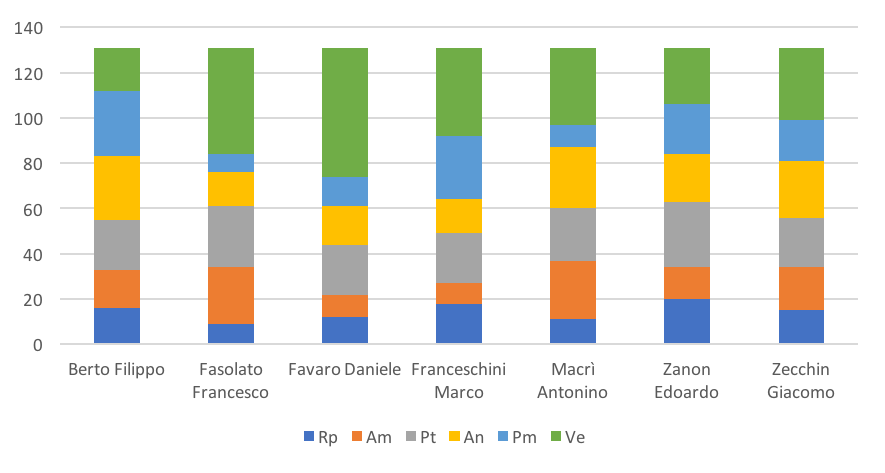
\includegraphics[width=\textwidth]{Preventivo/Immagini/totale_oreRuoloPersona.png}
				\caption{Riassunto ore totali di lavoro per persona}
			\end{figure}	
			
			\newpage
			\paragraph{Prospetto economico}
			Il costo di ogni ruolo è indicato di seguito:
			\begin{table}[h]
				\centering
				\begin{tabular}{l * {2}{c}}
				\toprule
				\textbf{Ruolo} & \textbf{Ore} & \textbf{Costo (\euro{})} \\
				\midrule
				Responsabile & 101 & 3.030,00 \\
				%\midrule
				Amministratore & 120 & 2.400,00 \\
				%\midrule
				Progettista & 167 & 3.674,00 \\
				%\midrule
				Analista & 148 & 3.700,00 \\		
				%\midrule
				Programmatore & 128 & 1.920,00 \\		
				%\midrule
				Verificatore & 253 & 3.795,00 \\				
				\midrule		
				\textbf{Totale} & 917 & 18.519,00 \\
				\bottomrule	
				\end{tabular}
				\caption{Prospetto economico totale}		
			\end{table}
			
			Riassumendo la precedente tabella con due pie chart:	
			\begin{figure}[!h]
				\centering
				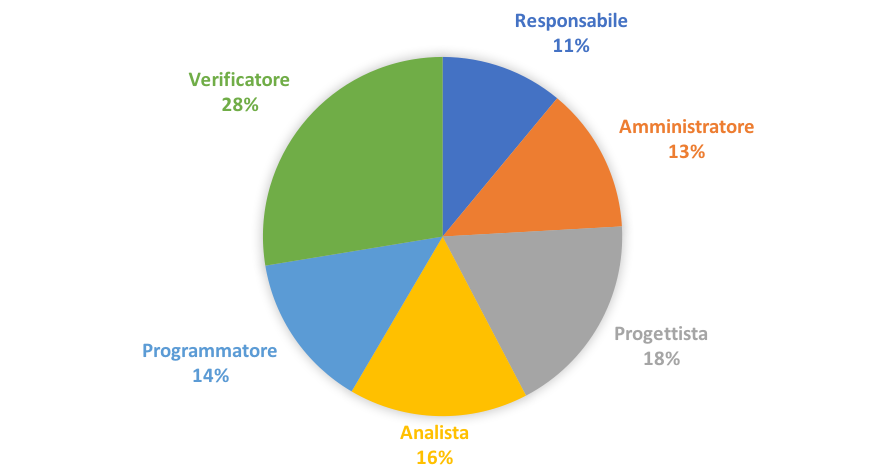
\includegraphics[width=\textwidth]{Preventivo/Immagini/totale_oreRuolo.png}
				\caption{Riassunto ore totali di lavoro per ruolo}
			\end{figure}	
			\newpage
			\begin{figure}[!h]
				\centering
				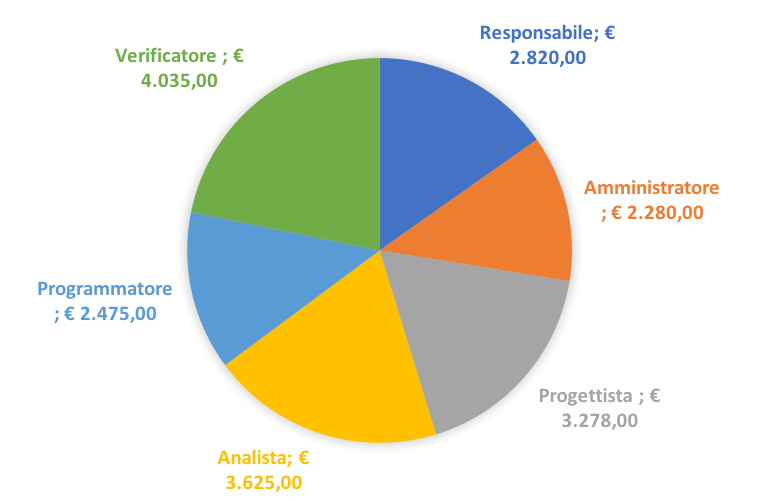
\includegraphics[width=\textwidth]{Preventivo/Immagini/totale_costoRuolo.png}
				\caption{Riassunto costo totale per ruolo}
			\end{figure}	

		\newpage
		\subsubsection{Ore di investimento}
			\paragraph{Suddivisione del lavoro}
			Ogni componente del gruppo \kpanic\ rivestirà i seguenti ruoli:
			\begin{table}[h]
				%\centering
				\begin{tabularx}{\textwidth}{l * {6}{C} c}
				\toprule
				\textbf{Nominativo} & \textbf{Rp} & \textbf{Am} & \textbf{Pt} & \textbf{An} & \textbf{Pm} & \textbf{Ve} & \textbf{Ore totali} \\
				\midrule
				Berto Filippo &	0 & 13 & 0 & 14 & 0 & 4 &  31 \\
				%\midrule
				Fasolato Francesco & 9 & 9 & 0 & 0 & 0 & 14 & 32 \\
				%\midrule
				Favaro Daniele & 14 & 0 & 0 & 0 & 13 & 0 & 35 \\
				%\midrule
				Franceschini Marco & 0 & 12 & 0 & 12 & 0 & 11 & 35 \\
				%\midrule
				Macrì Antonino & 11 & 8 & 0 & 9 & 0 & 8 & 36 \\
				%\midrule
				Zanon Edoardo &	0 & 14 & 0 & 16 & 0 & 5 & 35 \\
				%\midrule
				Zecchin Giacomo & 0 & 11 & 0 & 18 & 0 & 5 & 34 \\
				\midrule			
				\textbf{Ore Totali Ruolo} & 34 & 67 & 0 & 82 & 0 & 55 & 238 \\
				\bottomrule
				\end{tabularx}
				\caption{Suddivisione delle ore investite di lavoro}		
			\end{table}

			Riassumendo la precedente tabella con un bar chart:	
			\begin{figure}[!h]
				\centering
				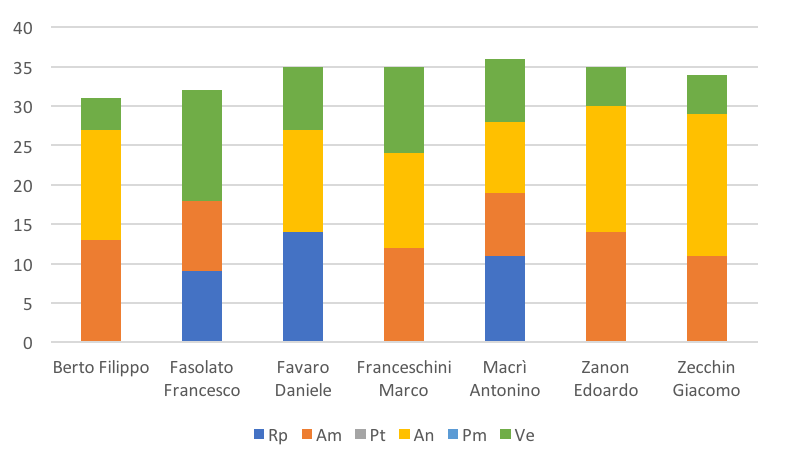
\includegraphics[width=\textwidth]{Preventivo//Immagini/investito_oreRuoloPersona.png}
				\caption{Riassunto ore di lavoro investite per persona}
			\end{figure}	
			
			\newpage
			\paragraph{Prospetto economico}
			Il costo di ogni ruolo è indicato di seguito:
			\begin{table}[h]
				\centering
				\begin{tabular}{l * {2}{c}}
				\toprule
				\textbf{Ruolo} & \textbf{Ore} & \textbf{Costo (\euro{})} \\
				\midrule
				Responsabile & 34 & 1.020,00 \\
				%\midrule
				Amministratore & 67 & 1.340,00 \\
				%\midrule
				Progettista & 0 & 0,00 \\
				%\midrule
				Analista & 82 & 2.050,00 \\		
				%\midrule
				Programmatore & 0 & 0,00 \\		
				%\midrule
				Verificatore & 55 & 825 ,00 \\				
				\midrule		
				\textbf{Totale} & 238 & 5.235,00 \\
				\bottomrule	
				\end{tabular}
				\caption{Prospetto economico investimento}		
			\end{table}
			
			Riassumendo la precedente tabella con due pie chart:	
			\begin{figure}[!h]
				\centering
				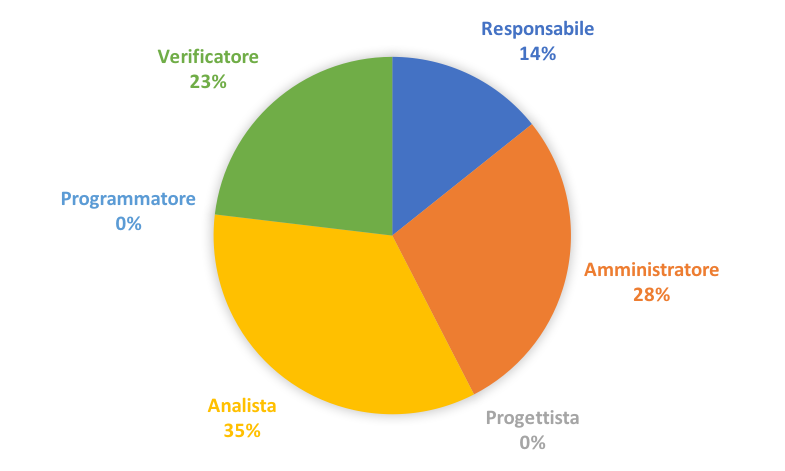
\includegraphics[width=\textwidth]{Preventivo/Immagini/investito_oreRuolo.png}
				\caption{Riassunto ore investite di lavoro per ruolo}
			\end{figure}	
			\newpage
			\begin{figure}[!h]
				\centering
				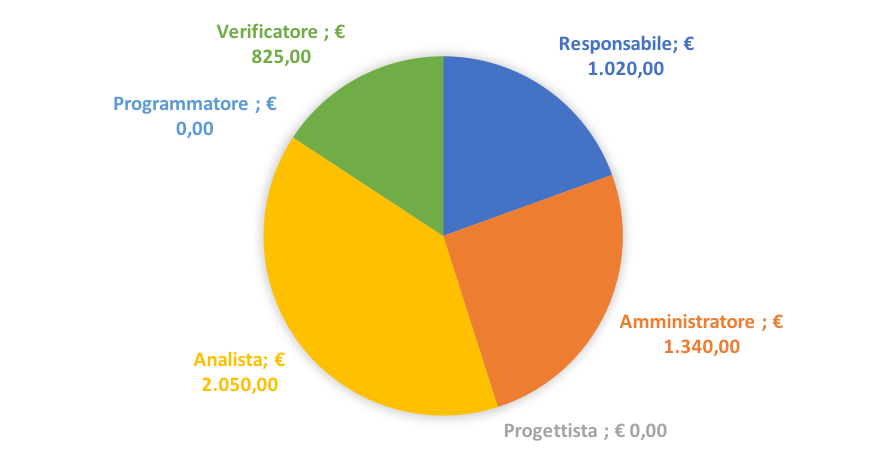
\includegraphics[width=\textwidth]{Preventivo/Immagini/investito_costoRuolo.png}
				\caption{Riassunto costo investimento per ruolo}
			\end{figure}
	
		\newpage
		\subsubsection{Ore rendicontate}
			\paragraph{Suddivisione del lavoro}
			Vengono riportate le ore totali che ogni componente del gruppo \kpanic\ dedicherà per ogni ruolo a rotazione:
			\begin{table}[h]
				%\centering
				\begin{tabularx}{\textwidth}{l * {6}{C} c}
				\toprule
				\textbf{Nominativo} & \textbf{Rp} & \textbf{Am} & \textbf{Pt} & \textbf{An} & \textbf{Pm} & \textbf{Ve} & \textbf{Ore totali} \\
				\midrule
				Berto Filippo &	16 & 4 & 22 & 16 & 29 & 14 & 131 \\
				%\midrule
				Fasolato Francesco & 0 & 16 & 27 & 15 & 8 & 35 & 131 \\
				%\midrule
				Favaro Daniele & 0 & 10 & 22 & 5 & 13 & 51 & 131 \\
				%\midrule
				Franceschini Marco & 18 & 0 & 22 & 3 & 28 & 30 & 131 \\
				%\midrule
				Macrì Antonino & 0 & 18 & 23 & 20 & 10 & 30 & 131 \\
				%\midrule
				Zanon Edoardo &	20 & 0 & 29 & 10 & 22 & 20 & 131 \\
				%\midrule
				Zecchin Giacomo & 15 & 8 & 22 & 11 & 18 & 27 & 131 \\
				\midrule			
				\textbf{Ore Totali Ruolo} & 69 & 56 & 167 & 80 & 128 & 207 & 707 \\
				\bottomrule
				\end{tabularx}
				\caption{Suddivisione delle ore totali di lavoro}		
			\end{table}

			Riassumendo la precedente tabella con un bar chart:
			\begin{figure}[!h]
				\centering
				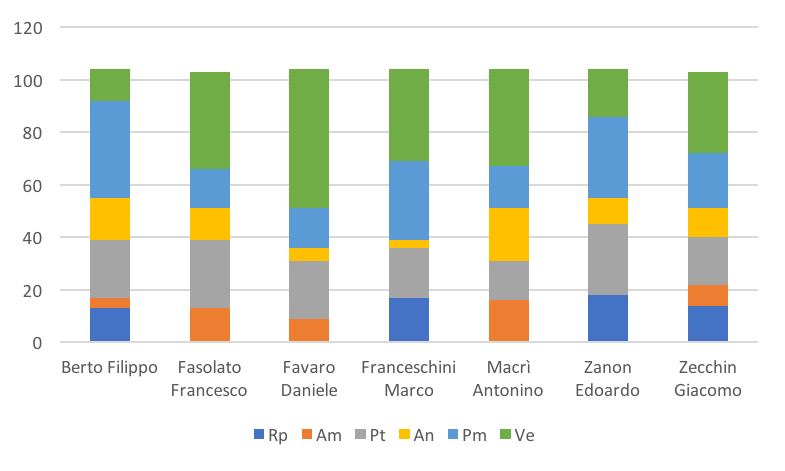
\includegraphics[width=\textwidth]{Preventivo/Immagini/rendicontato_oreRuoloPersona.png}
				\caption{Riassunto ore totali di lavoro per persona}
			\end{figure}	
			
			\newpage
			\paragraph{Prospetto economico}
			Il costo di ogni ruolo è indicato di seguito:
			\begin{table}[h]
				\centering
				\begin{tabular}{l * {2}{c}}
				\toprule
				\textbf{Ruolo} & \textbf{Ore} & \textbf{Costo (\euro{})} \\
				\midrule
				Responsabile & 69 & 2.070,00 \\
				%\midrule
				Amministratore & 56 & 1.120,00 \\
				%\midrule
				Progettista & 167 & 3.674,00 \\
				%\midrule
				Analista & 80 & 2.000,00 \\		
				%\midrule
				Programmatore & 128 & 1.920,00 \\		
				%\midrule
				Verificatore & 207 & 3.105,00 \\				
				\midrule		
				\textbf{Totale} & 707 & 13.889,00 \\
				\bottomrule	
				\end{tabular}
				\caption{Prospetto economico totale}		
			\end{table}
			
			Riassumendo la precedente tabella con due pie chart:	
			\begin{figure}[!h]
				\centering
				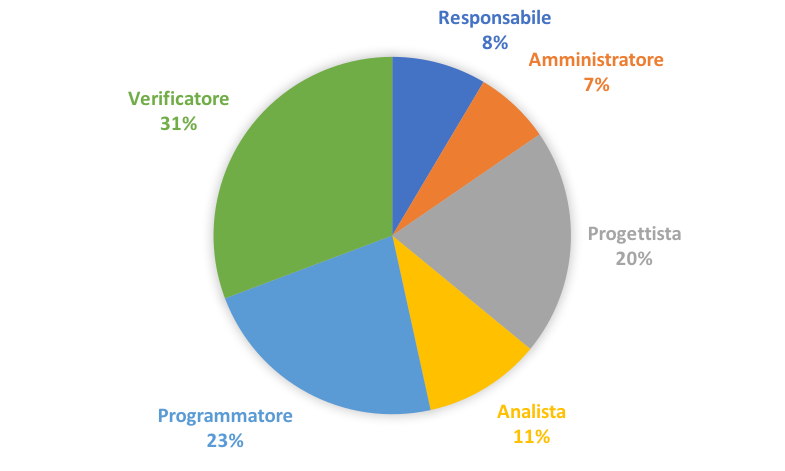
\includegraphics[width=\textwidth]{Preventivo/Immagini/rendicontato_oreRuolo.png}
				\caption{Riassunto ore totali di lavoro per ruolo}
			\end{figure}	
			\newpage
			\begin{figure}[!h]
				\centering
				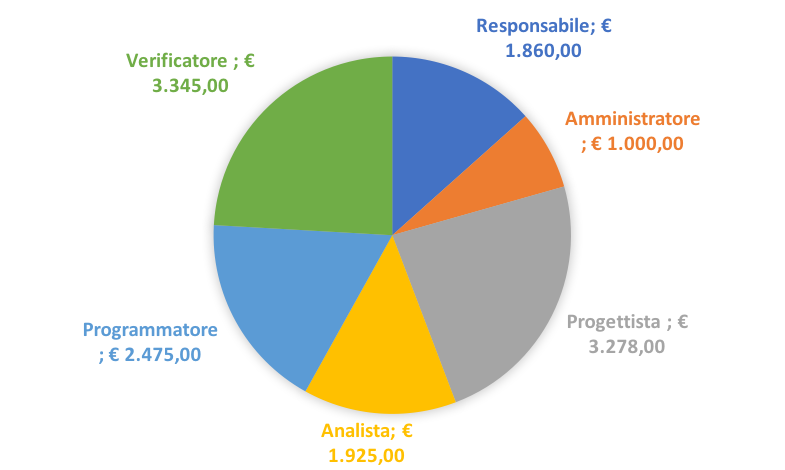
\includegraphics[width=\textwidth]{Preventivo/Immagini/rendicontato_costoRuolo.png}
				\caption{Riassunto costo totale per ruolo}
			\end{figure}

\end{document}